\documentclass[11pt]{article}
    \usepackage{ctex}
    \usepackage[breakable]{tcolorbox}
    \usepackage{parskip} % Stop auto-indenting (to mimic markdown behaviour)
    
    \usepackage{iftex}
    \ifPDFTeX
    	\usepackage[T1]{fontenc}
    	\usepackage{mathpazo}
    \else
    	\usepackage{fontspec}
    \fi

    % Basic figure setup, for now with no caption control since it's done
    % automatically by Pandoc (which extracts ![](path) syntax from Markdown).
    \usepackage{graphicx}
    % Maintain compatibility with old templates. Remove in nbconvert 6.0
    \let\Oldincludegraphics\includegraphics
    % Ensure that by default, figures have no caption (until we provide a
    % proper Figure object with a Caption API and a way to capture that
    % in the conversion process - todo).
    \usepackage{caption}
    \DeclareCaptionFormat{nocaption}{}
    \captionsetup{format=nocaption,aboveskip=0pt,belowskip=0pt}

    \usepackage[Export]{adjustbox} % Used to constrain images to a maximum size
    \adjustboxset{max size={0.9\linewidth}{0.9\paperheight}}
    \usepackage{float}
    \floatplacement{figure}{H} % forces figures to be placed at the correct location
    \usepackage{xcolor} % Allow colors to be defined
    \usepackage{enumerate} % Needed for markdown enumerations to work
    \usepackage{geometry} % Used to adjust the document margins
    \usepackage{amsmath} % Equations
    \usepackage{amssymb} % Equations
    \usepackage{textcomp} % defines textquotesingle
    % Hack from http://tex.stackexchange.com/a/47451/13684:
    \AtBeginDocument{%
        \def\PYZsq{\textquotesingle}% Upright quotes in Pygmentized code
    }
    \usepackage{upquote} % Upright quotes for verbatim code
    \usepackage{eurosym} % defines \euro
    \usepackage[mathletters]{ucs} % Extended unicode (utf-8) support
    \usepackage{fancyvrb} % verbatim replacement that allows latex
    \usepackage{grffile} % extends the file name processing of package graphics 
                         % to support a larger range
    \makeatletter % fix for grffile with XeLaTeX
    \def\Gread@@xetex#1{%
      \IfFileExists{"\Gin@base".bb}%
      {\Gread@eps{\Gin@base.bb}}%
      {\Gread@@xetex@aux#1}%
    }
    \makeatother

    % The hyperref package gives us a pdf with properly built
    % internal navigation ('pdf bookmarks' for the table of contents,
    % internal cross-reference links, web links for URLs, etc.)
    \usepackage{hyperref}
    % The default LaTeX title has an obnoxious amount of whitespace. By default,
    % titling removes some of it. It also provides customization options.
    \usepackage{titling}
    \usepackage{longtable} % longtable support required by pandoc >1.10
    \usepackage{booktabs}  % table support for pandoc > 1.12.2
    \usepackage[inline]{enumitem} % IRkernel/repr support (it uses the enumerate* environment)
    \usepackage[normalem]{ulem} % ulem is needed to support strikethroughs (\sout)
                                % normalem makes italics be italics, not underlines
    \usepackage{mathrsfs}
    

    
    % Colors for the hyperref package
    \definecolor{urlcolor}{rgb}{0,.145,.698}
    \definecolor{linkcolor}{rgb}{.71,0.21,0.01}
    \definecolor{citecolor}{rgb}{.12,.54,.11}

    % ANSI colors
    \definecolor{ansi-black}{HTML}{3E424D}
    \definecolor{ansi-black-intense}{HTML}{282C36}
    \definecolor{ansi-red}{HTML}{E75C58}
    \definecolor{ansi-red-intense}{HTML}{B22B31}
    \definecolor{ansi-green}{HTML}{00A250}
    \definecolor{ansi-green-intense}{HTML}{007427}
    \definecolor{ansi-yellow}{HTML}{DDB62B}
    \definecolor{ansi-yellow-intense}{HTML}{B27D12}
    \definecolor{ansi-blue}{HTML}{208FFB}
    \definecolor{ansi-blue-intense}{HTML}{0065CA}
    \definecolor{ansi-magenta}{HTML}{D160C4}
    \definecolor{ansi-magenta-intense}{HTML}{A03196}
    \definecolor{ansi-cyan}{HTML}{60C6C8}
    \definecolor{ansi-cyan-intense}{HTML}{258F8F}
    \definecolor{ansi-white}{HTML}{C5C1B4}
    \definecolor{ansi-white-intense}{HTML}{A1A6B2}
    \definecolor{ansi-default-inverse-fg}{HTML}{FFFFFF}
    \definecolor{ansi-default-inverse-bg}{HTML}{000000}

    % commands and environments needed by pandoc snippets
    % extracted from the output of `pandoc -s`
    \providecommand{\tightlist}{%
      \setlength{\itemsep}{0pt}\setlength{\parskip}{0pt}}
    \DefineVerbatimEnvironment{Highlighting}{Verbatim}{commandchars=\\\{\}}
    % Add ',fontsize=\small' for more characters per line
    \newenvironment{Shaded}{}{}
    \newcommand{\KeywordTok}[1]{\textcolor[rgb]{0.00,0.44,0.13}{\textbf{{#1}}}}
    \newcommand{\DataTypeTok}[1]{\textcolor[rgb]{0.56,0.13,0.00}{{#1}}}
    \newcommand{\DecValTok}[1]{\textcolor[rgb]{0.25,0.63,0.44}{{#1}}}
    \newcommand{\BaseNTok}[1]{\textcolor[rgb]{0.25,0.63,0.44}{{#1}}}
    \newcommand{\FloatTok}[1]{\textcolor[rgb]{0.25,0.63,0.44}{{#1}}}
    \newcommand{\CharTok}[1]{\textcolor[rgb]{0.25,0.44,0.63}{{#1}}}
    \newcommand{\StringTok}[1]{\textcolor[rgb]{0.25,0.44,0.63}{{#1}}}
    \newcommand{\CommentTok}[1]{\textcolor[rgb]{0.38,0.63,0.69}{\textit{{#1}}}}
    \newcommand{\OtherTok}[1]{\textcolor[rgb]{0.00,0.44,0.13}{{#1}}}
    \newcommand{\AlertTok}[1]{\textcolor[rgb]{1.00,0.00,0.00}{\textbf{{#1}}}}
    \newcommand{\FunctionTok}[1]{\textcolor[rgb]{0.02,0.16,0.49}{{#1}}}
    \newcommand{\RegionMarkerTok}[1]{{#1}}
    \newcommand{\ErrorTok}[1]{\textcolor[rgb]{1.00,0.00,0.00}{\textbf{{#1}}}}
    \newcommand{\NormalTok}[1]{{#1}}
    
    % Additional commands for more recent versions of Pandoc
    \newcommand{\ConstantTok}[1]{\textcolor[rgb]{0.53,0.00,0.00}{{#1}}}
    \newcommand{\SpecialCharTok}[1]{\textcolor[rgb]{0.25,0.44,0.63}{{#1}}}
    \newcommand{\VerbatimStringTok}[1]{\textcolor[rgb]{0.25,0.44,0.63}{{#1}}}
    \newcommand{\SpecialStringTok}[1]{\textcolor[rgb]{0.73,0.40,0.53}{{#1}}}
    \newcommand{\ImportTok}[1]{{#1}}
    \newcommand{\DocumentationTok}[1]{\textcolor[rgb]{0.73,0.13,0.13}{\textit{{#1}}}}
    \newcommand{\AnnotationTok}[1]{\textcolor[rgb]{0.38,0.63,0.69}{\textbf{\textit{{#1}}}}}
    \newcommand{\CommentVarTok}[1]{\textcolor[rgb]{0.38,0.63,0.69}{\textbf{\textit{{#1}}}}}
    \newcommand{\VariableTok}[1]{\textcolor[rgb]{0.10,0.09,0.49}{{#1}}}
    \newcommand{\ControlFlowTok}[1]{\textcolor[rgb]{0.00,0.44,0.13}{\textbf{{#1}}}}
    \newcommand{\OperatorTok}[1]{\textcolor[rgb]{0.40,0.40,0.40}{{#1}}}
    \newcommand{\BuiltInTok}[1]{{#1}}
    \newcommand{\ExtensionTok}[1]{{#1}}
    \newcommand{\PreprocessorTok}[1]{\textcolor[rgb]{0.74,0.48,0.00}{{#1}}}
    \newcommand{\AttributeTok}[1]{\textcolor[rgb]{0.49,0.56,0.16}{{#1}}}
    \newcommand{\InformationTok}[1]{\textcolor[rgb]{0.38,0.63,0.69}{\textbf{\textit{{#1}}}}}
    \newcommand{\WarningTok}[1]{\textcolor[rgb]{0.38,0.63,0.69}{\textbf{\textit{{#1}}}}}
    
    
    % Define a nice break command that doesn't care if a line doesn't already
    % exist.
    \def\br{\hspace*{\fill} \\* }
    % Math Jax compatibility definitions
    \def\gt{>}
    \def\lt{<}
    \let\Oldtex\TeX
    \let\Oldlatex\LaTeX
    \renewcommand{\TeX}{\textrm{\Oldtex}}
    \renewcommand{\LaTeX}{\textrm{\Oldlatex}}
    % Document parameters
    % Document title
    \title{lecture02}
    \author{Zeffiretti Hiesh}
    
    
    
    
    
% Pygments definitions
\makeatletter
\def\PY@reset{\let\PY@it=\relax \let\PY@bf=\relax%
    \let\PY@ul=\relax \let\PY@tc=\relax%
    \let\PY@bc=\relax \let\PY@ff=\relax}
\def\PY@tok#1{\csname PY@tok@#1\endcsname}
\def\PY@toks#1+{\ifx\relax#1\empty\else%
    \PY@tok{#1}\expandafter\PY@toks\fi}
\def\PY@do#1{\PY@bc{\PY@tc{\PY@ul{%
    \PY@it{\PY@bf{\PY@ff{#1}}}}}}}
\def\PY#1#2{\PY@reset\PY@toks#1+\relax+\PY@do{#2}}

\expandafter\def\csname PY@tok@w\endcsname{\def\PY@tc##1{\textcolor[rgb]{0.73,0.73,0.73}{##1}}}
\expandafter\def\csname PY@tok@c\endcsname{\let\PY@it=\textit\def\PY@tc##1{\textcolor[rgb]{0.25,0.50,0.50}{##1}}}
\expandafter\def\csname PY@tok@cp\endcsname{\def\PY@tc##1{\textcolor[rgb]{0.74,0.48,0.00}{##1}}}
\expandafter\def\csname PY@tok@k\endcsname{\let\PY@bf=\textbf\def\PY@tc##1{\textcolor[rgb]{0.00,0.50,0.00}{##1}}}
\expandafter\def\csname PY@tok@kp\endcsname{\def\PY@tc##1{\textcolor[rgb]{0.00,0.50,0.00}{##1}}}
\expandafter\def\csname PY@tok@kt\endcsname{\def\PY@tc##1{\textcolor[rgb]{0.69,0.00,0.25}{##1}}}
\expandafter\def\csname PY@tok@o\endcsname{\def\PY@tc##1{\textcolor[rgb]{0.40,0.40,0.40}{##1}}}
\expandafter\def\csname PY@tok@ow\endcsname{\let\PY@bf=\textbf\def\PY@tc##1{\textcolor[rgb]{0.67,0.13,1.00}{##1}}}
\expandafter\def\csname PY@tok@nb\endcsname{\def\PY@tc##1{\textcolor[rgb]{0.00,0.50,0.00}{##1}}}
\expandafter\def\csname PY@tok@nf\endcsname{\def\PY@tc##1{\textcolor[rgb]{0.00,0.00,1.00}{##1}}}
\expandafter\def\csname PY@tok@nc\endcsname{\let\PY@bf=\textbf\def\PY@tc##1{\textcolor[rgb]{0.00,0.00,1.00}{##1}}}
\expandafter\def\csname PY@tok@nn\endcsname{\let\PY@bf=\textbf\def\PY@tc##1{\textcolor[rgb]{0.00,0.00,1.00}{##1}}}
\expandafter\def\csname PY@tok@ne\endcsname{\let\PY@bf=\textbf\def\PY@tc##1{\textcolor[rgb]{0.82,0.25,0.23}{##1}}}
\expandafter\def\csname PY@tok@nv\endcsname{\def\PY@tc##1{\textcolor[rgb]{0.10,0.09,0.49}{##1}}}
\expandafter\def\csname PY@tok@no\endcsname{\def\PY@tc##1{\textcolor[rgb]{0.53,0.00,0.00}{##1}}}
\expandafter\def\csname PY@tok@nl\endcsname{\def\PY@tc##1{\textcolor[rgb]{0.63,0.63,0.00}{##1}}}
\expandafter\def\csname PY@tok@ni\endcsname{\let\PY@bf=\textbf\def\PY@tc##1{\textcolor[rgb]{0.60,0.60,0.60}{##1}}}
\expandafter\def\csname PY@tok@na\endcsname{\def\PY@tc##1{\textcolor[rgb]{0.49,0.56,0.16}{##1}}}
\expandafter\def\csname PY@tok@nt\endcsname{\let\PY@bf=\textbf\def\PY@tc##1{\textcolor[rgb]{0.00,0.50,0.00}{##1}}}
\expandafter\def\csname PY@tok@nd\endcsname{\def\PY@tc##1{\textcolor[rgb]{0.67,0.13,1.00}{##1}}}
\expandafter\def\csname PY@tok@s\endcsname{\def\PY@tc##1{\textcolor[rgb]{0.73,0.13,0.13}{##1}}}
\expandafter\def\csname PY@tok@sd\endcsname{\let\PY@it=\textit\def\PY@tc##1{\textcolor[rgb]{0.73,0.13,0.13}{##1}}}
\expandafter\def\csname PY@tok@si\endcsname{\let\PY@bf=\textbf\def\PY@tc##1{\textcolor[rgb]{0.73,0.40,0.53}{##1}}}
\expandafter\def\csname PY@tok@se\endcsname{\let\PY@bf=\textbf\def\PY@tc##1{\textcolor[rgb]{0.73,0.40,0.13}{##1}}}
\expandafter\def\csname PY@tok@sr\endcsname{\def\PY@tc##1{\textcolor[rgb]{0.73,0.40,0.53}{##1}}}
\expandafter\def\csname PY@tok@ss\endcsname{\def\PY@tc##1{\textcolor[rgb]{0.10,0.09,0.49}{##1}}}
\expandafter\def\csname PY@tok@sx\endcsname{\def\PY@tc##1{\textcolor[rgb]{0.00,0.50,0.00}{##1}}}
\expandafter\def\csname PY@tok@m\endcsname{\def\PY@tc##1{\textcolor[rgb]{0.40,0.40,0.40}{##1}}}
\expandafter\def\csname PY@tok@gh\endcsname{\let\PY@bf=\textbf\def\PY@tc##1{\textcolor[rgb]{0.00,0.00,0.50}{##1}}}
\expandafter\def\csname PY@tok@gu\endcsname{\let\PY@bf=\textbf\def\PY@tc##1{\textcolor[rgb]{0.50,0.00,0.50}{##1}}}
\expandafter\def\csname PY@tok@gd\endcsname{\def\PY@tc##1{\textcolor[rgb]{0.63,0.00,0.00}{##1}}}
\expandafter\def\csname PY@tok@gi\endcsname{\def\PY@tc##1{\textcolor[rgb]{0.00,0.63,0.00}{##1}}}
\expandafter\def\csname PY@tok@gr\endcsname{\def\PY@tc##1{\textcolor[rgb]{1.00,0.00,0.00}{##1}}}
\expandafter\def\csname PY@tok@ge\endcsname{\let\PY@it=\textit}
\expandafter\def\csname PY@tok@gs\endcsname{\let\PY@bf=\textbf}
\expandafter\def\csname PY@tok@gp\endcsname{\let\PY@bf=\textbf\def\PY@tc##1{\textcolor[rgb]{0.00,0.00,0.50}{##1}}}
\expandafter\def\csname PY@tok@go\endcsname{\def\PY@tc##1{\textcolor[rgb]{0.53,0.53,0.53}{##1}}}
\expandafter\def\csname PY@tok@gt\endcsname{\def\PY@tc##1{\textcolor[rgb]{0.00,0.27,0.87}{##1}}}
\expandafter\def\csname PY@tok@err\endcsname{\def\PY@bc##1{\setlength{\fboxsep}{0pt}\fcolorbox[rgb]{1.00,0.00,0.00}{1,1,1}{\strut ##1}}}
\expandafter\def\csname PY@tok@kc\endcsname{\let\PY@bf=\textbf\def\PY@tc##1{\textcolor[rgb]{0.00,0.50,0.00}{##1}}}
\expandafter\def\csname PY@tok@kd\endcsname{\let\PY@bf=\textbf\def\PY@tc##1{\textcolor[rgb]{0.00,0.50,0.00}{##1}}}
\expandafter\def\csname PY@tok@kn\endcsname{\let\PY@bf=\textbf\def\PY@tc##1{\textcolor[rgb]{0.00,0.50,0.00}{##1}}}
\expandafter\def\csname PY@tok@kr\endcsname{\let\PY@bf=\textbf\def\PY@tc##1{\textcolor[rgb]{0.00,0.50,0.00}{##1}}}
\expandafter\def\csname PY@tok@bp\endcsname{\def\PY@tc##1{\textcolor[rgb]{0.00,0.50,0.00}{##1}}}
\expandafter\def\csname PY@tok@fm\endcsname{\def\PY@tc##1{\textcolor[rgb]{0.00,0.00,1.00}{##1}}}
\expandafter\def\csname PY@tok@vc\endcsname{\def\PY@tc##1{\textcolor[rgb]{0.10,0.09,0.49}{##1}}}
\expandafter\def\csname PY@tok@vg\endcsname{\def\PY@tc##1{\textcolor[rgb]{0.10,0.09,0.49}{##1}}}
\expandafter\def\csname PY@tok@vi\endcsname{\def\PY@tc##1{\textcolor[rgb]{0.10,0.09,0.49}{##1}}}
\expandafter\def\csname PY@tok@vm\endcsname{\def\PY@tc##1{\textcolor[rgb]{0.10,0.09,0.49}{##1}}}
\expandafter\def\csname PY@tok@sa\endcsname{\def\PY@tc##1{\textcolor[rgb]{0.73,0.13,0.13}{##1}}}
\expandafter\def\csname PY@tok@sb\endcsname{\def\PY@tc##1{\textcolor[rgb]{0.73,0.13,0.13}{##1}}}
\expandafter\def\csname PY@tok@sc\endcsname{\def\PY@tc##1{\textcolor[rgb]{0.73,0.13,0.13}{##1}}}
\expandafter\def\csname PY@tok@dl\endcsname{\def\PY@tc##1{\textcolor[rgb]{0.73,0.13,0.13}{##1}}}
\expandafter\def\csname PY@tok@s2\endcsname{\def\PY@tc##1{\textcolor[rgb]{0.73,0.13,0.13}{##1}}}
\expandafter\def\csname PY@tok@sh\endcsname{\def\PY@tc##1{\textcolor[rgb]{0.73,0.13,0.13}{##1}}}
\expandafter\def\csname PY@tok@s1\endcsname{\def\PY@tc##1{\textcolor[rgb]{0.73,0.13,0.13}{##1}}}
\expandafter\def\csname PY@tok@mb\endcsname{\def\PY@tc##1{\textcolor[rgb]{0.40,0.40,0.40}{##1}}}
\expandafter\def\csname PY@tok@mf\endcsname{\def\PY@tc##1{\textcolor[rgb]{0.40,0.40,0.40}{##1}}}
\expandafter\def\csname PY@tok@mh\endcsname{\def\PY@tc##1{\textcolor[rgb]{0.40,0.40,0.40}{##1}}}
\expandafter\def\csname PY@tok@mi\endcsname{\def\PY@tc##1{\textcolor[rgb]{0.40,0.40,0.40}{##1}}}
\expandafter\def\csname PY@tok@il\endcsname{\def\PY@tc##1{\textcolor[rgb]{0.40,0.40,0.40}{##1}}}
\expandafter\def\csname PY@tok@mo\endcsname{\def\PY@tc##1{\textcolor[rgb]{0.40,0.40,0.40}{##1}}}
\expandafter\def\csname PY@tok@ch\endcsname{\let\PY@it=\textit\def\PY@tc##1{\textcolor[rgb]{0.25,0.50,0.50}{##1}}}
\expandafter\def\csname PY@tok@cm\endcsname{\let\PY@it=\textit\def\PY@tc##1{\textcolor[rgb]{0.25,0.50,0.50}{##1}}}
\expandafter\def\csname PY@tok@cpf\endcsname{\let\PY@it=\textit\def\PY@tc##1{\textcolor[rgb]{0.25,0.50,0.50}{##1}}}
\expandafter\def\csname PY@tok@c1\endcsname{\let\PY@it=\textit\def\PY@tc##1{\textcolor[rgb]{0.25,0.50,0.50}{##1}}}
\expandafter\def\csname PY@tok@cs\endcsname{\let\PY@it=\textit\def\PY@tc##1{\textcolor[rgb]{0.25,0.50,0.50}{##1}}}

\def\PYZbs{\char`\\}
\def\PYZus{\char`\_}
\def\PYZob{\char`\{}
\def\PYZcb{\char`\}}
\def\PYZca{\char`\^}
\def\PYZam{\char`\&}
\def\PYZlt{\char`\<}
\def\PYZgt{\char`\>}
\def\PYZsh{\char`\#}
\def\PYZpc{\char`\%}
\def\PYZdl{\char`\$}
\def\PYZhy{\char`\-}
\def\PYZsq{\char`\'}
\def\PYZdq{\char`\"}
\def\PYZti{\char`\~}
% for compatibility with earlier versions
\def\PYZat{@}
\def\PYZlb{[}
\def\PYZrb{]}
\makeatother


    % For linebreaks inside Verbatim environment from package fancyvrb. 
    \makeatletter
        \newbox\Wrappedcontinuationbox 
        \newbox\Wrappedvisiblespacebox 
        \newcommand*\Wrappedvisiblespace {\textcolor{red}{\textvisiblespace}} 
        \newcommand*\Wrappedcontinuationsymbol {\textcolor{red}{\llap{\tiny$\m@th\hookrightarrow$}}} 
        \newcommand*\Wrappedcontinuationindent {3ex } 
        \newcommand*\Wrappedafterbreak {\kern\Wrappedcontinuationindent\copy\Wrappedcontinuationbox} 
        % Take advantage of the already applied Pygments mark-up to insert 
        % potential linebreaks for TeX processing. 
        %        {, <, #, %, $, ' and ": go to next line. 
        %        _, }, ^, &, >, - and ~: stay at end of broken line. 
        % Use of \textquotesingle for straight quote. 
        \newcommand*\Wrappedbreaksatspecials {% 
            \def\PYGZus{\discretionary{\char`\_}{\Wrappedafterbreak}{\char`\_}}% 
            \def\PYGZob{\discretionary{}{\Wrappedafterbreak\char`\{}{\char`\{}}% 
            \def\PYGZcb{\discretionary{\char`\}}{\Wrappedafterbreak}{\char`\}}}% 
            \def\PYGZca{\discretionary{\char`\^}{\Wrappedafterbreak}{\char`\^}}% 
            \def\PYGZam{\discretionary{\char`\&}{\Wrappedafterbreak}{\char`\&}}% 
            \def\PYGZlt{\discretionary{}{\Wrappedafterbreak\char`\<}{\char`\<}}% 
            \def\PYGZgt{\discretionary{\char`\>}{\Wrappedafterbreak}{\char`\>}}% 
            \def\PYGZsh{\discretionary{}{\Wrappedafterbreak\char`\#}{\char`\#}}% 
            \def\PYGZpc{\discretionary{}{\Wrappedafterbreak\char`\%}{\char`\%}}% 
            \def\PYGZdl{\discretionary{}{\Wrappedafterbreak\char`\$}{\char`\$}}% 
            \def\PYGZhy{\discretionary{\char`\-}{\Wrappedafterbreak}{\char`\-}}% 
            \def\PYGZsq{\discretionary{}{\Wrappedafterbreak\textquotesingle}{\textquotesingle}}% 
            \def\PYGZdq{\discretionary{}{\Wrappedafterbreak\char`\"}{\char`\"}}% 
            \def\PYGZti{\discretionary{\char`\~}{\Wrappedafterbreak}{\char`\~}}% 
        } 
        % Some characters . , ; ? ! / are not pygmentized. 
        % This macro makes them "active" and they will insert potential linebreaks 
        \newcommand*\Wrappedbreaksatpunct {% 
            \lccode`\~`\.\lowercase{\def~}{\discretionary{\hbox{\char`\.}}{\Wrappedafterbreak}{\hbox{\char`\.}}}% 
            \lccode`\~`\,\lowercase{\def~}{\discretionary{\hbox{\char`\,}}{\Wrappedafterbreak}{\hbox{\char`\,}}}% 
            \lccode`\~`\;\lowercase{\def~}{\discretionary{\hbox{\char`\;}}{\Wrappedafterbreak}{\hbox{\char`\;}}}% 
            \lccode`\~`\:\lowercase{\def~}{\discretionary{\hbox{\char`\:}}{\Wrappedafterbreak}{\hbox{\char`\:}}}% 
            \lccode`\~`\?\lowercase{\def~}{\discretionary{\hbox{\char`\?}}{\Wrappedafterbreak}{\hbox{\char`\?}}}% 
            \lccode`\~`\!\lowercase{\def~}{\discretionary{\hbox{\char`\!}}{\Wrappedafterbreak}{\hbox{\char`\!}}}% 
            \lccode`\~`\/\lowercase{\def~}{\discretionary{\hbox{\char`\/}}{\Wrappedafterbreak}{\hbox{\char`\/}}}% 
            \catcode`\.\active
            \catcode`\,\active 
            \catcode`\;\active
            \catcode`\:\active
            \catcode`\?\active
            \catcode`\!\active
            \catcode`\/\active 
            \lccode`\~`\~ 	
        }
    \makeatother

    \let\OriginalVerbatim=\Verbatim
    \makeatletter
    \renewcommand{\Verbatim}[1][1]{%
        %\parskip\z@skip
        \sbox\Wrappedcontinuationbox {\Wrappedcontinuationsymbol}%
        \sbox\Wrappedvisiblespacebox {\FV@SetupFont\Wrappedvisiblespace}%
        \def\FancyVerbFormatLine ##1{\hsize\linewidth
            \vtop{\raggedright\hyphenpenalty\z@\exhyphenpenalty\z@
                \doublehyphendemerits\z@\finalhyphendemerits\z@
                \strut ##1\strut}%
        }%
        % If the linebreak is at a space, the latter will be displayed as visible
        % space at end of first line, and a continuation symbol starts next line.
        % Stretch/shrink are however usually zero for typewriter font.
        \def\FV@Space {%
            \nobreak\hskip\z@ plus\fontdimen3\font minus\fontdimen4\font
            \discretionary{\copy\Wrappedvisiblespacebox}{\Wrappedafterbreak}
            {\kern\fontdimen2\font}%
        }%
        
        % Allow breaks at special characters using \PYG... macros.
        \Wrappedbreaksatspecials
        % Breaks at punctuation characters . , ; ? ! and / need catcode=\active 	
        \OriginalVerbatim[#1,codes*=\Wrappedbreaksatpunct]%
    }
    \makeatother

    % Exact colors from NB
    \definecolor{incolor}{HTML}{303F9F}
    \definecolor{outcolor}{HTML}{D84315}
    \definecolor{cellborder}{HTML}{CFCFCF}
    \definecolor{cellbackground}{HTML}{F7F7F7}
    
    % prompt
    \makeatletter
    \newcommand{\boxspacing}{\kern\kvtcb@left@rule\kern\kvtcb@boxsep}
    \makeatother
    \newcommand{\prompt}[4]{
        \ttfamily\llap{{\color{#2}[#3]:\hspace{3pt}#4}}\vspace{-\baselineskip}
    }
    

    
    % Prevent overflowing lines due to hard-to-break entities
    \sloppy 
    % Setup hyperref package
    \hypersetup{
      breaklinks=true,  % so long urls are correctly broken across lines
      colorlinks=true,
      urlcolor=urlcolor,
      linkcolor=linkcolor,
      citecolor=citecolor,
      }
    % Slightly bigger margins than the latex defaults
    
    \geometry{verbose,tmargin=1in,bmargin=1in,lmargin=1in,rmargin=1in}
    
    

\begin{document}
    
    \maketitle
    
    

    
    \hypertarget{lagrangian-v.s.-eulerian-two-views-of-continuums}{%
\subsubsection{Lagrangian v.s. Eulerian: Two Views of
Continuums}\label{lagrangian-v.s.-eulerian-two-views-of-continuums}}

\begin{enumerate}
\def\labelenumi{\arabic{enumi}.}
\tightlist
\item
  Lagrangian View, 拉格朗日视角:

  \begin{itemize}
  \tightlist
  \item
    Sensors that move passively with the simulated material(随波逐流)
  \item
    粒子
  \end{itemize}
\item
  Eulerian View, 欧拉视角:

  \begin{itemize}
  \tightlist
  \item
    Still sensors that never moves.(岿然不动)
  \item
    网格
  \end{itemize}
\end{enumerate}

    \hypertarget{mass-spring-system-ux5f39ux7c27-ux8d28ux70b9ux6a21ux578b}{%
\subsubsection{Mass-Spring System,
弹簧-质点模型}\label{mass-spring-system-ux5f39ux7c27-ux8d28ux70b9ux6a21ux578b}}

\begin{itemize}
\tightlist
\item
  Extremely ordinary
\item
  But very useful!

  \begin{itemize}
  \tightlist
  \item
    Cloth
  \item
    Elastic objects
  \item
    \ldots{}
  \end{itemize}
\end{itemize}

\hypertarget{mathematical-model}{%
\paragraph{Mathematical Model}\label{mathematical-model}}

\begin{equation*}
\begin{array}{rll}
    {\rm f}_ {ij} &=-k(||{\rm x}_ {i}-{\rm x}_ {j}||_ {2}- l_{ij})(\widehat{{\rm x}_ {i}-{\rm x}_ {j}})&(Hooke's Law) \\
    {\rm f}_ {i} &= \displaystyle\sum_{j}^{j\ne i}{\rm f}_ {ij}  & \\
    \displaystyle\frac{\partial {\rm v}}{\partial t} &= \displaystyle\frac{1}{m_{i}}{\rm f}_ {i} &
\end{array}
\end{equation*}

\(k\): spring stiffness;

\(l_{ij}\): spring rest length between particle \(i\) and particle
\(j\);

\(m_{i}\): the mass of particle \(i\).

\((\widehat{{\rm x}_ {i}-{\rm x}_ {j}})\): direction vector from
particle \(i\) to particle \(j\);

\hypertarget{time-integration}{%
\paragraph{Time integration}\label{time-integration}}

\begin{itemize}
\tightlist
\item
  Forward Euler (explicit)
\end{itemize}

\begin{equation*}
\begin{array}{rl}
    {\rm v}_ {t+1} &={\rm v}_ {t}+\Delta t\displaystyle\frac{{\rm f}_ {t}}{m} \\
    {\rm x}_ {t+1} &={\rm x}_ {t}+\Delta t{\rm v}_{t}
\end{array}
\end{equation*}

\begin{itemize}
\tightlist
\item
  Semi-implicit Euler (aka. sympletic Euler, explicit)
\end{itemize}

\begin{equation*}
\begin{array}{rl}
    {\rm v}_ {t+1} &= {\rm v}_ {t}+\Delta t\displaystyle\frac{{\rm f}_ {t+1}}{m} \\
    {\rm x}_ {t+1} &= {\rm x}_ {t}+\Delta t{\rm v}_{t+1}
\end{array}
\end{equation*}

\begin{itemize}
\tightlist
\item
  Backward Euler (often with Newton's method, implicit)
\end{itemize}

Implementing a mass-spring system with sympletic Euler

Steps: 1. Compute new velocity using
\({\rm v} {t+1}={\rm v}_ {t}+ \Delta t \frac{{\rm f}_{t}}{m}\) 2.
Collision with ground 3. Compute new position using
\({\rm x}_ {t+1}={\rm x}_ {t}+ \Delta t {\rm v}_ {t_1}\)

    \begin{tcolorbox}[breakable, size=fbox, boxrule=1pt, pad at break*=1mm,colback=cellbackground, colframe=cellborder]
\prompt{In}{incolor}{ }{\boxspacing}
\begin{Verbatim}[commandchars=\\\{\}]
\PY{c+c1}{\PYZsh{} Showcase}
\PY{c+c1}{\PYZsh{} Tutorials (Chinese):}
\PY{c+c1}{\PYZsh{} \PYZhy{} https://www.bilibili.com/video/BV1UK4y177iH}
\PY{c+c1}{\PYZsh{} \PYZhy{} https://www.bilibili.com/video/BV1DK411A771}

\PY{k+kn}{import} \PY{n+nn}{taichi} \PY{k}{as} \PY{n+nn}{ti}

\PY{n}{ti}\PY{o}{.}\PY{n}{init}\PY{p}{(}\PY{n}{arch}\PY{o}{=}\PY{n}{ti}\PY{o}{.}\PY{n}{gpu}\PY{p}{)}

\PY{n}{spring\PYZus{}Y} \PY{o}{=} \PY{n}{ti}\PY{o}{.}\PY{n}{field}\PY{p}{(}\PY{n}{dtype}\PY{o}{=}\PY{n}{ti}\PY{o}{.}\PY{n}{f32}\PY{p}{,} \PY{n}{shape}\PY{o}{=}\PY{p}{(}\PY{p}{)}\PY{p}{)}  \PY{c+c1}{\PYZsh{} Young\PYZsq{}s modulus}
\PY{n}{paused} \PY{o}{=} \PY{n}{ti}\PY{o}{.}\PY{n}{field}\PY{p}{(}\PY{n}{dtype}\PY{o}{=}\PY{n}{ti}\PY{o}{.}\PY{n}{i32}\PY{p}{,} \PY{n}{shape}\PY{o}{=}\PY{p}{(}\PY{p}{)}\PY{p}{)}
\PY{n}{drag\PYZus{}damping} \PY{o}{=} \PY{n}{ti}\PY{o}{.}\PY{n}{field}\PY{p}{(}\PY{n}{dtype}\PY{o}{=}\PY{n}{ti}\PY{o}{.}\PY{n}{f32}\PY{p}{,} \PY{n}{shape}\PY{o}{=}\PY{p}{(}\PY{p}{)}\PY{p}{)}
\PY{n}{dashpot\PYZus{}damping} \PY{o}{=} \PY{n}{ti}\PY{o}{.}\PY{n}{field}\PY{p}{(}\PY{n}{dtype}\PY{o}{=}\PY{n}{ti}\PY{o}{.}\PY{n}{f32}\PY{p}{,} \PY{n}{shape}\PY{o}{=}\PY{p}{(}\PY{p}{)}\PY{p}{)}

\PY{n}{max\PYZus{}num\PYZus{}particles} \PY{o}{=} \PY{l+m+mi}{1024}
\PY{n}{particle\PYZus{}mass} \PY{o}{=} \PY{l+m+mf}{1.0}
\PY{n}{dt} \PY{o}{=} \PY{l+m+mf}{1e\PYZhy{}3}
\PY{n}{substeps} \PY{o}{=} \PY{l+m+mi}{10}

\PY{n}{num\PYZus{}particles} \PY{o}{=} \PY{n}{ti}\PY{o}{.}\PY{n}{field}\PY{p}{(}\PY{n}{dtype}\PY{o}{=}\PY{n}{ti}\PY{o}{.}\PY{n}{i32}\PY{p}{,} \PY{n}{shape}\PY{o}{=}\PY{p}{(}\PY{p}{)}\PY{p}{)}
\PY{n}{x} \PY{o}{=} \PY{n}{ti}\PY{o}{.}\PY{n}{Vector}\PY{o}{.}\PY{n}{field}\PY{p}{(}\PY{l+m+mi}{2}\PY{p}{,} \PY{n}{dtype}\PY{o}{=}\PY{n}{ti}\PY{o}{.}\PY{n}{f32}\PY{p}{,} \PY{n}{shape}\PY{o}{=}\PY{n}{max\PYZus{}num\PYZus{}particles}\PY{p}{)}
\PY{n}{v} \PY{o}{=} \PY{n}{ti}\PY{o}{.}\PY{n}{Vector}\PY{o}{.}\PY{n}{field}\PY{p}{(}\PY{l+m+mi}{2}\PY{p}{,} \PY{n}{dtype}\PY{o}{=}\PY{n}{ti}\PY{o}{.}\PY{n}{f32}\PY{p}{,} \PY{n}{shape}\PY{o}{=}\PY{n}{max\PYZus{}num\PYZus{}particles}\PY{p}{)}
\PY{n}{f} \PY{o}{=} \PY{n}{ti}\PY{o}{.}\PY{n}{Vector}\PY{o}{.}\PY{n}{field}\PY{p}{(}\PY{l+m+mi}{2}\PY{p}{,} \PY{n}{dtype}\PY{o}{=}\PY{n}{ti}\PY{o}{.}\PY{n}{f32}\PY{p}{,} \PY{n}{shape}\PY{o}{=}\PY{n}{max\PYZus{}num\PYZus{}particles}\PY{p}{)}
\PY{n}{fixed} \PY{o}{=} \PY{n}{ti}\PY{o}{.}\PY{n}{field}\PY{p}{(}\PY{n}{dtype}\PY{o}{=}\PY{n}{ti}\PY{o}{.}\PY{n}{i32}\PY{p}{,} \PY{n}{shape}\PY{o}{=}\PY{n}{max\PYZus{}num\PYZus{}particles}\PY{p}{)}

\PY{c+c1}{\PYZsh{} rest\PYZus{}length[i, j] == 0 means i and j are NOT connected}
\PY{n}{rest\PYZus{}length} \PY{o}{=} \PY{n}{ti}\PY{o}{.}\PY{n}{field}\PY{p}{(}\PY{n}{dtype}\PY{o}{=}\PY{n}{ti}\PY{o}{.}\PY{n}{f32}\PY{p}{,}
                       \PY{n}{shape}\PY{o}{=}\PY{p}{(}\PY{n}{max\PYZus{}num\PYZus{}particles}\PY{p}{,} \PY{n}{max\PYZus{}num\PYZus{}particles}\PY{p}{)}\PY{p}{)}


\PY{n+nd}{@ti}\PY{o}{.}\PY{n}{kernel}
\PY{k}{def} \PY{n+nf}{substep}\PY{p}{(}\PY{p}{)}\PY{p}{:}
    \PY{n}{n} \PY{o}{=} \PY{n}{num\PYZus{}particles}\PY{p}{[}\PY{k+kc}{None}\PY{p}{]}

    \PY{c+c1}{\PYZsh{} Compute force}
    \PY{k}{for} \PY{n}{i} \PY{o+ow}{in} \PY{n+nb}{range}\PY{p}{(}\PY{n}{n}\PY{p}{)}\PY{p}{:}
        \PY{c+c1}{\PYZsh{} Gravity}
        \PY{n}{f}\PY{p}{[}\PY{n}{i}\PY{p}{]} \PY{o}{=} \PY{n}{ti}\PY{o}{.}\PY{n}{Vector}\PY{p}{(}\PY{p}{[}\PY{l+m+mi}{0}\PY{p}{,} \PY{o}{\PYZhy{}}\PY{l+m+mf}{9.8}\PY{p}{]}\PY{p}{)} \PY{o}{*} \PY{n}{particle\PYZus{}mass}
        \PY{k}{for} \PY{n}{j} \PY{o+ow}{in} \PY{n+nb}{range}\PY{p}{(}\PY{n}{n}\PY{p}{)}\PY{p}{:}
            \PY{k}{if} \PY{n}{rest\PYZus{}length}\PY{p}{[}\PY{n}{i}\PY{p}{,} \PY{n}{j}\PY{p}{]} \PY{o}{!=} \PY{l+m+mi}{0}\PY{p}{:}
                \PY{n}{x\PYZus{}ij} \PY{o}{=} \PY{n}{x}\PY{p}{[}\PY{n}{i}\PY{p}{]} \PY{o}{\PYZhy{}} \PY{n}{x}\PY{p}{[}\PY{n}{j}\PY{p}{]}
                \PY{n}{d} \PY{o}{=} \PY{n}{x\PYZus{}ij}\PY{o}{.}\PY{n}{normalized}\PY{p}{(}\PY{p}{)}

                \PY{c+c1}{\PYZsh{} Spring force}
                \PY{n}{f}\PY{p}{[}\PY{n}{i}\PY{p}{]} \PY{o}{+}\PY{o}{=} \PY{o}{\PYZhy{}}\PY{n}{spring\PYZus{}Y}\PY{p}{[}\PY{k+kc}{None}\PY{p}{]} \PY{o}{*} \PY{p}{(}\PY{n}{x\PYZus{}ij}\PY{o}{.}\PY{n}{norm}\PY{p}{(}\PY{p}{)} \PY{o}{/} \PY{n}{rest\PYZus{}length}\PY{p}{[}\PY{n}{i}\PY{p}{,} \PY{n}{j}\PY{p}{]} \PY{o}{\PYZhy{}}
                                           \PY{l+m+mi}{1}\PY{p}{)} \PY{o}{*} \PY{n}{d}

                \PY{c+c1}{\PYZsh{} Dashpot damping}
                \PY{n}{v\PYZus{}rel} \PY{o}{=} \PY{p}{(}\PY{n}{v}\PY{p}{[}\PY{n}{i}\PY{p}{]} \PY{o}{\PYZhy{}} \PY{n}{v}\PY{p}{[}\PY{n}{j}\PY{p}{]}\PY{p}{)}\PY{o}{.}\PY{n}{dot}\PY{p}{(}\PY{n}{d}\PY{p}{)}
                \PY{n}{f}\PY{p}{[}\PY{n}{i}\PY{p}{]} \PY{o}{+}\PY{o}{=} \PY{o}{\PYZhy{}}\PY{n}{dashpot\PYZus{}damping}\PY{p}{[}\PY{k+kc}{None}\PY{p}{]} \PY{o}{*} \PY{n}{v\PYZus{}rel} \PY{o}{*} \PY{n}{d}

    \PY{c+c1}{\PYZsh{} We use a semi\PYZhy{}implicit Euler (aka symplectic Euler) time integrator}
    \PY{k}{for} \PY{n}{i} \PY{o+ow}{in} \PY{n+nb}{range}\PY{p}{(}\PY{n}{n}\PY{p}{)}\PY{p}{:}
        \PY{k}{if} \PY{o+ow}{not} \PY{n}{fixed}\PY{p}{[}\PY{n}{i}\PY{p}{]}\PY{p}{:}
            \PY{n}{v}\PY{p}{[}\PY{n}{i}\PY{p}{]} \PY{o}{+}\PY{o}{=} \PY{n}{dt} \PY{o}{*} \PY{n}{f}\PY{p}{[}\PY{n}{i}\PY{p}{]} \PY{o}{/} \PY{n}{particle\PYZus{}mass}
            \PY{n}{v}\PY{p}{[}\PY{n}{i}\PY{p}{]} \PY{o}{*}\PY{o}{=} \PY{n}{ti}\PY{o}{.}\PY{n}{exp}\PY{p}{(}\PY{o}{\PYZhy{}}\PY{n}{dt} \PY{o}{*} \PY{n}{drag\PYZus{}damping}\PY{p}{[}\PY{k+kc}{None}\PY{p}{]}\PY{p}{)}  \PY{c+c1}{\PYZsh{} Drag damping}

            \PY{n}{x}\PY{p}{[}\PY{n}{i}\PY{p}{]} \PY{o}{+}\PY{o}{=} \PY{n}{v}\PY{p}{[}\PY{n}{i}\PY{p}{]} \PY{o}{*} \PY{n}{dt}
        \PY{k}{else}\PY{p}{:}
            \PY{n}{v}\PY{p}{[}\PY{n}{i}\PY{p}{]} \PY{o}{=} \PY{n}{ti}\PY{o}{.}\PY{n}{Vector}\PY{p}{(}\PY{p}{[}\PY{l+m+mi}{0}\PY{p}{,} \PY{l+m+mi}{0}\PY{p}{]}\PY{p}{)}

        \PY{c+c1}{\PYZsh{} Collide with four walls}
        \PY{k}{for} \PY{n}{d} \PY{o+ow}{in} \PY{n}{ti}\PY{o}{.}\PY{n}{static}\PY{p}{(}\PY{n+nb}{range}\PY{p}{(}\PY{l+m+mi}{2}\PY{p}{)}\PY{p}{)}\PY{p}{:}
            \PY{c+c1}{\PYZsh{} d = 0: treating X (horizontal) component}
            \PY{c+c1}{\PYZsh{} d = 1: treating Y (vertical) component}

            \PY{k}{if} \PY{n}{x}\PY{p}{[}\PY{n}{i}\PY{p}{]}\PY{p}{[}\PY{n}{d}\PY{p}{]} \PY{o}{\PYZlt{}} \PY{l+m+mi}{0}\PY{p}{:}  \PY{c+c1}{\PYZsh{} Bottom and left}
                \PY{n}{x}\PY{p}{[}\PY{n}{i}\PY{p}{]}\PY{p}{[}\PY{n}{d}\PY{p}{]} \PY{o}{=} \PY{l+m+mi}{0}  \PY{c+c1}{\PYZsh{} move particle inside}
                \PY{n}{v}\PY{p}{[}\PY{n}{i}\PY{p}{]}\PY{p}{[}\PY{n}{d}\PY{p}{]} \PY{o}{=} \PY{l+m+mi}{0}  \PY{c+c1}{\PYZsh{} stop it from moving further}

            \PY{k}{if} \PY{n}{x}\PY{p}{[}\PY{n}{i}\PY{p}{]}\PY{p}{[}\PY{n}{d}\PY{p}{]} \PY{o}{\PYZgt{}} \PY{l+m+mi}{1}\PY{p}{:}  \PY{c+c1}{\PYZsh{} Top and right}
                \PY{n}{x}\PY{p}{[}\PY{n}{i}\PY{p}{]}\PY{p}{[}\PY{n}{d}\PY{p}{]} \PY{o}{=} \PY{l+m+mi}{1}  \PY{c+c1}{\PYZsh{} move particle inside}
                \PY{n}{v}\PY{p}{[}\PY{n}{i}\PY{p}{]}\PY{p}{[}\PY{n}{d}\PY{p}{]} \PY{o}{=} \PY{l+m+mi}{0}  \PY{c+c1}{\PYZsh{} stop it from moving further}


\PY{n+nd}{@ti}\PY{o}{.}\PY{n}{kernel}
\PY{k}{def} \PY{n+nf}{new\PYZus{}particle}\PY{p}{(}\PY{n}{pos\PYZus{}x}\PY{p}{:} \PY{n}{ti}\PY{o}{.}\PY{n}{f32}\PY{p}{,} \PY{n}{pos\PYZus{}y}\PY{p}{:} \PY{n}{ti}\PY{o}{.}\PY{n}{f32}\PY{p}{,} \PY{n}{fixed\PYZus{}}\PY{p}{:} \PY{n}{ti}\PY{o}{.}\PY{n}{i32}\PY{p}{)}\PY{p}{:}
    \PY{c+c1}{\PYZsh{} Taichi doesn\PYZsq{}t support using vectors as kernel arguments yet, so we pass scalars}
    \PY{n}{new\PYZus{}particle\PYZus{}id} \PY{o}{=} \PY{n}{num\PYZus{}particles}\PY{p}{[}\PY{k+kc}{None}\PY{p}{]}
    \PY{n}{x}\PY{p}{[}\PY{n}{new\PYZus{}particle\PYZus{}id}\PY{p}{]} \PY{o}{=} \PY{p}{[}\PY{n}{pos\PYZus{}x}\PY{p}{,} \PY{n}{pos\PYZus{}y}\PY{p}{]}
    \PY{n}{v}\PY{p}{[}\PY{n}{new\PYZus{}particle\PYZus{}id}\PY{p}{]} \PY{o}{=} \PY{p}{[}\PY{l+m+mi}{0}\PY{p}{,} \PY{l+m+mi}{0}\PY{p}{]}
    \PY{n}{fixed}\PY{p}{[}\PY{n}{new\PYZus{}particle\PYZus{}id}\PY{p}{]} \PY{o}{=} \PY{n}{fixed\PYZus{}}
    \PY{n}{num\PYZus{}particles}\PY{p}{[}\PY{k+kc}{None}\PY{p}{]} \PY{o}{+}\PY{o}{=} \PY{l+m+mi}{1}

    \PY{c+c1}{\PYZsh{} Connect with existing particles}
    \PY{k}{for} \PY{n}{i} \PY{o+ow}{in} \PY{n+nb}{range}\PY{p}{(}\PY{n}{new\PYZus{}particle\PYZus{}id}\PY{p}{)}\PY{p}{:}
        \PY{n}{dist} \PY{o}{=} \PY{p}{(}\PY{n}{x}\PY{p}{[}\PY{n}{new\PYZus{}particle\PYZus{}id}\PY{p}{]} \PY{o}{\PYZhy{}} \PY{n}{x}\PY{p}{[}\PY{n}{i}\PY{p}{]}\PY{p}{)}\PY{o}{.}\PY{n}{norm}\PY{p}{(}\PY{p}{)}
        \PY{n}{connection\PYZus{}radius} \PY{o}{=} \PY{l+m+mf}{0.15}
        \PY{k}{if} \PY{n}{dist} \PY{o}{\PYZlt{}} \PY{n}{connection\PYZus{}radius}\PY{p}{:}
            \PY{c+c1}{\PYZsh{} Connect the new particle with particle i}
            \PY{n}{rest\PYZus{}length}\PY{p}{[}\PY{n}{i}\PY{p}{,} \PY{n}{new\PYZus{}particle\PYZus{}id}\PY{p}{]} \PY{o}{=} \PY{l+m+mf}{0.1}
            \PY{n}{rest\PYZus{}length}\PY{p}{[}\PY{n}{new\PYZus{}particle\PYZus{}id}\PY{p}{,} \PY{n}{i}\PY{p}{]} \PY{o}{=} \PY{l+m+mf}{0.1}


\PY{n+nd}{@ti}\PY{o}{.}\PY{n}{kernel}
\PY{k}{def} \PY{n+nf}{attract}\PY{p}{(}\PY{n}{pos\PYZus{}x}\PY{p}{:} \PY{n}{ti}\PY{o}{.}\PY{n}{f32}\PY{p}{,} \PY{n}{pos\PYZus{}y}\PY{p}{:} \PY{n}{ti}\PY{o}{.}\PY{n}{f32}\PY{p}{)}\PY{p}{:}
    \PY{k}{for} \PY{n}{i} \PY{o+ow}{in} \PY{n+nb}{range}\PY{p}{(}\PY{n}{num\PYZus{}particles}\PY{p}{[}\PY{k+kc}{None}\PY{p}{]}\PY{p}{)}\PY{p}{:}
        \PY{n}{p} \PY{o}{=} \PY{n}{ti}\PY{o}{.}\PY{n}{Vector}\PY{p}{(}\PY{p}{[}\PY{n}{pos\PYZus{}x}\PY{p}{,} \PY{n}{pos\PYZus{}y}\PY{p}{]}\PY{p}{)}
        \PY{n}{v}\PY{p}{[}\PY{n}{i}\PY{p}{]} \PY{o}{+}\PY{o}{=} \PY{o}{\PYZhy{}}\PY{n}{dt} \PY{o}{*} \PY{n}{substeps} \PY{o}{*} \PY{p}{(}\PY{n}{x}\PY{p}{[}\PY{n}{i}\PY{p}{]} \PY{o}{\PYZhy{}} \PY{n}{p}\PY{p}{)} \PY{o}{*} \PY{l+m+mi}{100}


\PY{k}{def} \PY{n+nf}{main}\PY{p}{(}\PY{p}{)}\PY{p}{:}
    \PY{n}{gui} \PY{o}{=} \PY{n}{ti}\PY{o}{.}\PY{n}{GUI}\PY{p}{(}\PY{l+s+s1}{\PYZsq{}}\PY{l+s+s1}{Explicit Mass Spring System}\PY{l+s+s1}{\PYZsq{}}\PY{p}{,}
                 \PY{n}{res}\PY{o}{=}\PY{p}{(}\PY{l+m+mi}{512}\PY{p}{,} \PY{l+m+mi}{512}\PY{p}{)}\PY{p}{,}
                 \PY{n}{background\PYZus{}color}\PY{o}{=}\PY{l+m+mh}{0xDDDDDD}\PY{p}{)}

    \PY{n}{spring\PYZus{}Y}\PY{p}{[}\PY{k+kc}{None}\PY{p}{]} \PY{o}{=} \PY{l+m+mi}{1000}
    \PY{n}{drag\PYZus{}damping}\PY{p}{[}\PY{k+kc}{None}\PY{p}{]} \PY{o}{=} \PY{l+m+mi}{1}
    \PY{n}{dashpot\PYZus{}damping}\PY{p}{[}\PY{k+kc}{None}\PY{p}{]} \PY{o}{=} \PY{l+m+mi}{100}

    \PY{n}{new\PYZus{}particle}\PY{p}{(}\PY{l+m+mf}{0.3}\PY{p}{,} \PY{l+m+mf}{0.3}\PY{p}{,} \PY{k+kc}{False}\PY{p}{)}
    \PY{n}{new\PYZus{}particle}\PY{p}{(}\PY{l+m+mf}{0.3}\PY{p}{,} \PY{l+m+mf}{0.4}\PY{p}{,} \PY{k+kc}{False}\PY{p}{)}
    \PY{n}{new\PYZus{}particle}\PY{p}{(}\PY{l+m+mf}{0.4}\PY{p}{,} \PY{l+m+mf}{0.4}\PY{p}{,} \PY{k+kc}{False}\PY{p}{)}

    \PY{k}{while} \PY{k+kc}{True}\PY{p}{:}
        \PY{k}{for} \PY{n}{e} \PY{o+ow}{in} \PY{n}{gui}\PY{o}{.}\PY{n}{get\PYZus{}events}\PY{p}{(}\PY{n}{ti}\PY{o}{.}\PY{n}{GUI}\PY{o}{.}\PY{n}{PRESS}\PY{p}{)}\PY{p}{:}
            \PY{k}{if} \PY{n}{e}\PY{o}{.}\PY{n}{key} \PY{o+ow}{in} \PY{p}{[}\PY{n}{ti}\PY{o}{.}\PY{n}{GUI}\PY{o}{.}\PY{n}{ESCAPE}\PY{p}{,} \PY{n}{ti}\PY{o}{.}\PY{n}{GUI}\PY{o}{.}\PY{n}{EXIT}\PY{p}{]}\PY{p}{:}
                \PY{n}{exit}\PY{p}{(}\PY{p}{)}
            \PY{k}{elif} \PY{n}{e}\PY{o}{.}\PY{n}{key} \PY{o}{==} \PY{n}{gui}\PY{o}{.}\PY{n}{SPACE}\PY{p}{:}
                \PY{n}{paused}\PY{p}{[}\PY{k+kc}{None}\PY{p}{]} \PY{o}{=} \PY{o+ow}{not} \PY{n}{paused}\PY{p}{[}\PY{k+kc}{None}\PY{p}{]}
            \PY{k}{elif} \PY{n}{e}\PY{o}{.}\PY{n}{key} \PY{o}{==} \PY{n}{ti}\PY{o}{.}\PY{n}{GUI}\PY{o}{.}\PY{n}{LMB}\PY{p}{:}
                \PY{n}{new\PYZus{}particle}\PY{p}{(}\PY{n}{e}\PY{o}{.}\PY{n}{pos}\PY{p}{[}\PY{l+m+mi}{0}\PY{p}{]}\PY{p}{,} \PY{n}{e}\PY{o}{.}\PY{n}{pos}\PY{p}{[}\PY{l+m+mi}{1}\PY{p}{]}\PY{p}{,}
                             \PY{n+nb}{int}\PY{p}{(}\PY{n}{gui}\PY{o}{.}\PY{n}{is\PYZus{}pressed}\PY{p}{(}\PY{n}{ti}\PY{o}{.}\PY{n}{GUI}\PY{o}{.}\PY{n}{SHIFT}\PY{p}{)}\PY{p}{)}\PY{p}{)}
            \PY{k}{elif} \PY{n}{e}\PY{o}{.}\PY{n}{key} \PY{o}{==} \PY{l+s+s1}{\PYZsq{}}\PY{l+s+s1}{c}\PY{l+s+s1}{\PYZsq{}}\PY{p}{:}
                \PY{n}{num\PYZus{}particles}\PY{p}{[}\PY{k+kc}{None}\PY{p}{]} \PY{o}{=} \PY{l+m+mi}{0}
                \PY{n}{rest\PYZus{}length}\PY{o}{.}\PY{n}{fill}\PY{p}{(}\PY{l+m+mi}{0}\PY{p}{)}
            \PY{k}{elif} \PY{n}{e}\PY{o}{.}\PY{n}{key} \PY{o}{==} \PY{l+s+s1}{\PYZsq{}}\PY{l+s+s1}{y}\PY{l+s+s1}{\PYZsq{}}\PY{p}{:}
                \PY{k}{if} \PY{n}{gui}\PY{o}{.}\PY{n}{is\PYZus{}pressed}\PY{p}{(}\PY{l+s+s1}{\PYZsq{}}\PY{l+s+s1}{Shift}\PY{l+s+s1}{\PYZsq{}}\PY{p}{)}\PY{p}{:}
                    \PY{n}{spring\PYZus{}Y}\PY{p}{[}\PY{k+kc}{None}\PY{p}{]} \PY{o}{/}\PY{o}{=} \PY{l+m+mf}{1.1}
                \PY{k}{else}\PY{p}{:}
                    \PY{n}{spring\PYZus{}Y}\PY{p}{[}\PY{k+kc}{None}\PY{p}{]} \PY{o}{*}\PY{o}{=} \PY{l+m+mf}{1.1}
            \PY{k}{elif} \PY{n}{e}\PY{o}{.}\PY{n}{key} \PY{o}{==} \PY{l+s+s1}{\PYZsq{}}\PY{l+s+s1}{d}\PY{l+s+s1}{\PYZsq{}}\PY{p}{:}
                \PY{k}{if} \PY{n}{gui}\PY{o}{.}\PY{n}{is\PYZus{}pressed}\PY{p}{(}\PY{l+s+s1}{\PYZsq{}}\PY{l+s+s1}{Shift}\PY{l+s+s1}{\PYZsq{}}\PY{p}{)}\PY{p}{:}
                    \PY{n}{drag\PYZus{}damping}\PY{p}{[}\PY{k+kc}{None}\PY{p}{]} \PY{o}{/}\PY{o}{=} \PY{l+m+mf}{1.1}
                \PY{k}{else}\PY{p}{:}
                    \PY{n}{drag\PYZus{}damping}\PY{p}{[}\PY{k+kc}{None}\PY{p}{]} \PY{o}{*}\PY{o}{=} \PY{l+m+mf}{1.1}
            \PY{k}{elif} \PY{n}{e}\PY{o}{.}\PY{n}{key} \PY{o}{==} \PY{l+s+s1}{\PYZsq{}}\PY{l+s+s1}{x}\PY{l+s+s1}{\PYZsq{}}\PY{p}{:}
                \PY{k}{if} \PY{n}{gui}\PY{o}{.}\PY{n}{is\PYZus{}pressed}\PY{p}{(}\PY{l+s+s1}{\PYZsq{}}\PY{l+s+s1}{Shift}\PY{l+s+s1}{\PYZsq{}}\PY{p}{)}\PY{p}{:}
                    \PY{n}{dashpot\PYZus{}damping}\PY{p}{[}\PY{k+kc}{None}\PY{p}{]} \PY{o}{/}\PY{o}{=} \PY{l+m+mf}{1.1}
                \PY{k}{else}\PY{p}{:}
                    \PY{n}{dashpot\PYZus{}damping}\PY{p}{[}\PY{k+kc}{None}\PY{p}{]} \PY{o}{*}\PY{o}{=} \PY{l+m+mf}{1.1}

        \PY{k}{if} \PY{n}{gui}\PY{o}{.}\PY{n}{is\PYZus{}pressed}\PY{p}{(}\PY{n}{ti}\PY{o}{.}\PY{n}{GUI}\PY{o}{.}\PY{n}{RMB}\PY{p}{)}\PY{p}{:}
            \PY{n}{cursor\PYZus{}pos} \PY{o}{=} \PY{n}{gui}\PY{o}{.}\PY{n}{get\PYZus{}cursor\PYZus{}pos}\PY{p}{(}\PY{p}{)}
            \PY{n}{attract}\PY{p}{(}\PY{n}{cursor\PYZus{}pos}\PY{p}{[}\PY{l+m+mi}{0}\PY{p}{]}\PY{p}{,} \PY{n}{cursor\PYZus{}pos}\PY{p}{[}\PY{l+m+mi}{1}\PY{p}{]}\PY{p}{)}

        \PY{k}{if} \PY{o+ow}{not} \PY{n}{paused}\PY{p}{[}\PY{k+kc}{None}\PY{p}{]}\PY{p}{:}
            \PY{k}{for} \PY{n}{step} \PY{o+ow}{in} \PY{n+nb}{range}\PY{p}{(}\PY{n}{substeps}\PY{p}{)}\PY{p}{:}
                \PY{n}{substep}\PY{p}{(}\PY{p}{)}

        \PY{n}{X} \PY{o}{=} \PY{n}{x}\PY{o}{.}\PY{n}{to\PYZus{}numpy}\PY{p}{(}\PY{p}{)}
        \PY{n}{n} \PY{o}{=} \PY{n}{num\PYZus{}particles}\PY{p}{[}\PY{k+kc}{None}\PY{p}{]}

        \PY{c+c1}{\PYZsh{} Draw the springs}
        \PY{k}{for} \PY{n}{i} \PY{o+ow}{in} \PY{n+nb}{range}\PY{p}{(}\PY{n}{n}\PY{p}{)}\PY{p}{:}
            \PY{k}{for} \PY{n}{j} \PY{o+ow}{in} \PY{n+nb}{range}\PY{p}{(}\PY{n}{i} \PY{o}{+} \PY{l+m+mi}{1}\PY{p}{,} \PY{n}{n}\PY{p}{)}\PY{p}{:}
                \PY{k}{if} \PY{n}{rest\PYZus{}length}\PY{p}{[}\PY{n}{i}\PY{p}{,} \PY{n}{j}\PY{p}{]} \PY{o}{!=} \PY{l+m+mi}{0}\PY{p}{:}
                    \PY{n}{gui}\PY{o}{.}\PY{n}{line}\PY{p}{(}\PY{n}{begin}\PY{o}{=}\PY{n}{X}\PY{p}{[}\PY{n}{i}\PY{p}{]}\PY{p}{,} \PY{n}{end}\PY{o}{=}\PY{n}{X}\PY{p}{[}\PY{n}{j}\PY{p}{]}\PY{p}{,} \PY{n}{radius}\PY{o}{=}\PY{l+m+mi}{2}\PY{p}{,} \PY{n}{color}\PY{o}{=}\PY{l+m+mh}{0x444444}\PY{p}{)}

        \PY{c+c1}{\PYZsh{} Draw the particles}
        \PY{k}{for} \PY{n}{i} \PY{o+ow}{in} \PY{n+nb}{range}\PY{p}{(}\PY{n}{n}\PY{p}{)}\PY{p}{:}
            \PY{n}{c} \PY{o}{=} \PY{l+m+mh}{0xFF0000} \PY{k}{if} \PY{n}{fixed}\PY{p}{[}\PY{n}{i}\PY{p}{]} \PY{k}{else} \PY{l+m+mh}{0x111111}
            \PY{n}{gui}\PY{o}{.}\PY{n}{circle}\PY{p}{(}\PY{n}{pos}\PY{o}{=}\PY{n}{X}\PY{p}{[}\PY{n}{i}\PY{p}{]}\PY{p}{,} \PY{n}{color}\PY{o}{=}\PY{n}{c}\PY{p}{,} \PY{n}{radius}\PY{o}{=}\PY{l+m+mi}{5}\PY{p}{)}

        \PY{n}{gui}\PY{o}{.}\PY{n}{text}\PY{p}{(}
            \PY{n}{content}\PY{o}{=}
            \PY{l+s+sa}{f}\PY{l+s+s1}{\PYZsq{}}\PY{l+s+s1}{Left click: add mass point (with shift to fix); Right click: attract}\PY{l+s+s1}{\PYZsq{}}\PY{p}{,}
            \PY{n}{pos}\PY{o}{=}\PY{p}{(}\PY{l+m+mi}{0}\PY{p}{,} \PY{l+m+mf}{0.99}\PY{p}{)}\PY{p}{,}
            \PY{n}{color}\PY{o}{=}\PY{l+m+mh}{0x0}\PY{p}{)}
        \PY{n}{gui}\PY{o}{.}\PY{n}{text}\PY{p}{(}\PY{n}{content}\PY{o}{=}\PY{l+s+sa}{f}\PY{l+s+s1}{\PYZsq{}}\PY{l+s+s1}{C: clear all; Space: pause}\PY{l+s+s1}{\PYZsq{}}\PY{p}{,}
                 \PY{n}{pos}\PY{o}{=}\PY{p}{(}\PY{l+m+mi}{0}\PY{p}{,} \PY{l+m+mf}{0.95}\PY{p}{)}\PY{p}{,}
                 \PY{n}{color}\PY{o}{=}\PY{l+m+mh}{0x0}\PY{p}{)}
        \PY{n}{gui}\PY{o}{.}\PY{n}{text}\PY{p}{(}\PY{n}{content}\PY{o}{=}\PY{l+s+sa}{f}\PY{l+s+s1}{\PYZsq{}}\PY{l+s+s1}{Y: Spring Young}\PY{l+s+se}{\PYZbs{}\PYZsq{}}\PY{l+s+s1}{s modulus }\PY{l+s+si}{\PYZob{}}\PY{n}{spring\PYZus{}Y}\PY{p}{[}\PY{k+kc}{None}\PY{p}{]}\PY{l+s+si}{:}\PY{l+s+s1}{.1f}\PY{l+s+si}{\PYZcb{}}\PY{l+s+s1}{\PYZsq{}}\PY{p}{,}
                 \PY{n}{pos}\PY{o}{=}\PY{p}{(}\PY{l+m+mi}{0}\PY{p}{,} \PY{l+m+mf}{0.9}\PY{p}{)}\PY{p}{,}
                 \PY{n}{color}\PY{o}{=}\PY{l+m+mh}{0x0}\PY{p}{)}
        \PY{n}{gui}\PY{o}{.}\PY{n}{text}\PY{p}{(}\PY{n}{content}\PY{o}{=}\PY{l+s+sa}{f}\PY{l+s+s1}{\PYZsq{}}\PY{l+s+s1}{D: Drag damping }\PY{l+s+si}{\PYZob{}}\PY{n}{drag\PYZus{}damping}\PY{p}{[}\PY{k+kc}{None}\PY{p}{]}\PY{l+s+si}{:}\PY{l+s+s1}{.2f}\PY{l+s+si}{\PYZcb{}}\PY{l+s+s1}{\PYZsq{}}\PY{p}{,}
                 \PY{n}{pos}\PY{o}{=}\PY{p}{(}\PY{l+m+mi}{0}\PY{p}{,} \PY{l+m+mf}{0.85}\PY{p}{)}\PY{p}{,}
                 \PY{n}{color}\PY{o}{=}\PY{l+m+mh}{0x0}\PY{p}{)}
        \PY{n}{gui}\PY{o}{.}\PY{n}{text}\PY{p}{(}\PY{n}{content}\PY{o}{=}\PY{l+s+sa}{f}\PY{l+s+s1}{\PYZsq{}}\PY{l+s+s1}{X: Dashpot damping }\PY{l+s+si}{\PYZob{}}\PY{n}{dashpot\PYZus{}damping}\PY{p}{[}\PY{k+kc}{None}\PY{p}{]}\PY{l+s+si}{:}\PY{l+s+s1}{.2f}\PY{l+s+si}{\PYZcb{}}\PY{l+s+s1}{\PYZsq{}}\PY{p}{,}
                 \PY{n}{pos}\PY{o}{=}\PY{p}{(}\PY{l+m+mi}{0}\PY{p}{,} \PY{l+m+mf}{0.8}\PY{p}{)}\PY{p}{,}
                 \PY{n}{color}\PY{o}{=}\PY{l+m+mh}{0x0}\PY{p}{)}
        \PY{n}{gui}\PY{o}{.}\PY{n}{show}\PY{p}{(}\PY{p}{)}


\PY{k}{if} \PY{n+nv+vm}{\PYZus{}\PYZus{}name\PYZus{}\PYZus{}} \PY{o}{==} \PY{l+s+s1}{\PYZsq{}}\PY{l+s+s1}{\PYZus{}\PYZus{}main\PYZus{}\PYZus{}}\PY{l+s+s1}{\PYZsq{}}\PY{p}{:}
    \PY{n}{main}\PY{p}{(}\PY{p}{)}
\end{Verbatim}
\end{tcolorbox}

    \hypertarget{explicit-v.s.-implicit-time-integrators}{%
\paragraph{Explicit v.s. implicit time
integrators}\label{explicit-v.s.-implicit-time-integrators}}

\begin{itemize}
\tightlist
\item
  Explicit (forward Euler, sympletic Euler, RK, \ldots):

  \begin{itemize}
  \tightlist
  \item
    Feature depends only on past
  \item
    Easy to implement
  \item
    Easy to explode: \(\Delta t \le c\sqrt{m/k}\), \((c\sim 1)\)
  \item
    Bad for stiff materials
  \end{itemize}
\item
  Implicit (backword Euler, middle-point, \ldots):

  \begin{itemize}
  \tightlist
  \item
    Future denpends on both future and past
  \item
    Chicken-egg problem: need to solve a system of (linear) equations
  \item
    Ingeneral harder to implement
  \item
    Each step is more expensive but time steps are larger

    \begin{itemize}
    \tightlist
    \item
      Sometimes brings you benefits
    \item
      \ldots{} but sometimes not
    \end{itemize}
  \item
    Numerical damping and locking
  \end{itemize}
\end{itemize}

\hypertarget{implementing}{%
\paragraph{Implementing}\label{implementing}}

\begin{itemize}
\tightlist
\item
  Implicit time integration:
\end{itemize}

\begin{equation*}
\begin{array}{rl}
    {\rm x}_ {t+1} &= {\rm x}_ {t}+\Delta t{\rm v}_ {t+1} \\
    {\rm v}_ {t+1} &= {\rm v}_ {t}+\Delta t{\rm M^{-1}f}({\rm x}_{t+1})
\end{array}
\end{equation*} - Eliminate \({\rm x}_ {t+1}\):

\begin{equation*}
    {\rm v}_ {t+1} = {\rm v}_ {t}+\Delta t{\rm M^{-1}f}{({\rm x}_ {t}+\Delta t{\rm v}_ {t+1})} \\
\end{equation*} - Linearize (one step of Newton's method):

\begin{equation*}
    {\rm v}_ {t+1} = {\rm v}_ {t}+\Delta t{\rm M^{-1}}\left[{{\rm f}({\rm x}_ {t})+\displaystyle\frac{\partial{\rm f}}{\partial {\rm x}}({\rm x}_ {t}) \Delta t{\rm v}_ {t+1}} \right]
\end{equation*}

\begin{equation*}
    \left[ {\rm I}-\Delta t^{2}{\rm M^{-1}}\displaystyle\frac{\partial{\rm f}}{\partial{\rm x}}({\rm x}_ {t})\right]{\rm v}_ {t+1}={\rm v}_ {t}\Delta t{\rm M^{-1}f}({\rm x}_{t})
\end{equation*}

How to solve it?

\begin{equation*}
\begin{array}{rl}
    A &= {\rm I}-\Delta t^{2}{\rm M^{-1}}\displaystyle\frac{\partial{\rm f}}{\partial{\rm x}}({\rm x}_ {t}) \\
    b &= {\rm v}_ {t}\Delta t{\rm M^{-1}f}({\rm x}_{t}) \\
    A{\rm v}_ {t+1} &= b
\end{array}
\end{equation*}

雅可比迭代法

对于矩阵 \(Ax=b\), \(A\)非奇异,且对角元不为0,可以将原方程组改写为:

\begin{equation*}
\left\{  
             \begin{array}{lr}  
             x_{1}=\displaystyle\frac{1}{a_{11}}\left(b_{1}-a_{11}x_{2}-...-a_{1n}x_{n}\right), &  \\  
             x_{2}=\displaystyle\frac{1}{a_{22}}\left(b_{2}-a_{21}x_{1}-...-a_{2n}x_{n}\right), & \\ 
             ...... & \\ 
             x_{n}=\displaystyle\frac{1}{a_{nn}}\left(b_{n}-a_{n1}x_{1}-...-a_{(n,n-1)}x_{n-1}\right), &   
             \end{array}  
\right.
\end{equation*}

    \begin{tcolorbox}[breakable, size=fbox, boxrule=1pt, pad at break*=1mm,colback=cellbackground, colframe=cellborder]
\prompt{In}{incolor}{ }{\boxspacing}
\begin{Verbatim}[commandchars=\\\{\}]
\PY{k+kn}{import} \PY{n+nn}{taichi} \PY{k}{as} \PY{n+nn}{ti}
\PY{k+kn}{import} \PY{n+nn}{random}

\PY{n}{ti}\PY{o}{.}\PY{n}{init}\PY{p}{(}\PY{n}{arch}\PY{o}{=}\PY{n}{ti}\PY{o}{.}\PY{n}{cpu}\PY{p}{)}

\PY{n}{n} \PY{o}{=} \PY{l+m+mi}{20}

\PY{n}{A} \PY{o}{=} \PY{n}{ti}\PY{o}{.}\PY{n}{field}\PY{p}{(}\PY{n}{dtype}\PY{o}{=}\PY{n}{ti}\PY{o}{.}\PY{n}{f32}\PY{p}{,} \PY{n}{shape}\PY{o}{=}\PY{p}{(}\PY{n}{n}\PY{p}{,} \PY{n}{n}\PY{p}{)}\PY{p}{)}
\PY{n}{x} \PY{o}{=} \PY{n}{ti}\PY{o}{.}\PY{n}{field}\PY{p}{(}\PY{n}{dtype}\PY{o}{=}\PY{n}{ti}\PY{o}{.}\PY{n}{f32}\PY{p}{,} \PY{n}{shape}\PY{o}{=}\PY{n}{n}\PY{p}{)}
\PY{n}{new\PYZus{}x} \PY{o}{=} \PY{n}{ti}\PY{o}{.}\PY{n}{field}\PY{p}{(}\PY{n}{dtype}\PY{o}{=}\PY{n}{ti}\PY{o}{.}\PY{n}{f32}\PY{p}{,} \PY{n}{shape}\PY{o}{=}\PY{n}{n}\PY{p}{)}
\PY{n}{b} \PY{o}{=} \PY{n}{ti}\PY{o}{.}\PY{n}{field}\PY{p}{(}\PY{n}{dtype}\PY{o}{=}\PY{n}{ti}\PY{o}{.}\PY{n}{f32}\PY{p}{,} \PY{n}{shape}\PY{o}{=}\PY{n}{n}\PY{p}{)}


\PY{c+c1}{\PYZsh{} 单步雅可比迭代}
\PY{n+nd}{@ti}\PY{o}{.}\PY{n}{kernel}
\PY{k}{def} \PY{n+nf}{iterate}\PY{p}{(}\PY{p}{)}\PY{p}{:}
    \PY{k}{for} \PY{n}{i} \PY{o+ow}{in} \PY{n+nb}{range}\PY{p}{(}\PY{n}{n}\PY{p}{)}\PY{p}{:}
        \PY{n}{r} \PY{o}{=} \PY{n}{b}\PY{p}{[}\PY{n}{i}\PY{p}{]}
        \PY{k}{for} \PY{n}{j} \PY{o+ow}{in} \PY{n+nb}{range}\PY{p}{(}\PY{n}{n}\PY{p}{)}\PY{p}{:}
            \PY{k}{if} \PY{n}{i} \PY{o}{!=} \PY{n}{j}\PY{p}{:}
                \PY{n}{r} \PY{o}{\PYZhy{}}\PY{o}{=} \PY{n}{A}\PY{p}{[}\PY{n}{i}\PY{p}{,} \PY{n}{j}\PY{p}{]} \PY{o}{*} \PY{n}{x}\PY{p}{[}\PY{n}{j}\PY{p}{]}

        \PY{n}{new\PYZus{}x}\PY{p}{[}\PY{n}{i}\PY{p}{]} \PY{o}{=} \PY{n}{r} \PY{o}{/} \PY{n}{A}\PY{p}{[}\PY{n}{i}\PY{p}{,} \PY{n}{i}\PY{p}{]}

    \PY{k}{for} \PY{n}{i} \PY{o+ow}{in} \PY{n+nb}{range}\PY{p}{(}\PY{n}{n}\PY{p}{)}\PY{p}{:}
        \PY{n}{x}\PY{p}{[}\PY{n}{i}\PY{p}{]} \PY{o}{=} \PY{n}{new\PYZus{}x}\PY{p}{[}\PY{n}{i}\PY{p}{]}


\PY{c+c1}{\PYZsh{} 计算误差}
\PY{n+nd}{@ti}\PY{o}{.}\PY{n}{kernel}
\PY{k}{def} \PY{n+nf}{residual}\PY{p}{(}\PY{p}{)} \PY{o}{\PYZhy{}}\PY{o}{\PYZgt{}} \PY{n}{ti}\PY{o}{.}\PY{n}{f32}\PY{p}{:}
    \PY{n}{res} \PY{o}{=} \PY{l+m+mf}{0.0}

    \PY{k}{for} \PY{n}{i} \PY{o+ow}{in} \PY{n+nb}{range}\PY{p}{(}\PY{n}{n}\PY{p}{)}\PY{p}{:}
        \PY{n}{r} \PY{o}{=} \PY{n}{b}\PY{p}{[}\PY{n}{i}\PY{p}{]} \PY{o}{*} \PY{l+m+mf}{1.0}
        \PY{k}{for} \PY{n}{j} \PY{o+ow}{in} \PY{n+nb}{range}\PY{p}{(}\PY{n}{n}\PY{p}{)}\PY{p}{:}
            \PY{n}{r} \PY{o}{\PYZhy{}}\PY{o}{=} \PY{n}{A}\PY{p}{[}\PY{n}{i}\PY{p}{,} \PY{n}{j}\PY{p}{]} \PY{o}{*} \PY{n}{x}\PY{p}{[}\PY{n}{j}\PY{p}{]}
        \PY{n}{res} \PY{o}{+}\PY{o}{=} \PY{n}{r} \PY{o}{*} \PY{n}{r}

    \PY{k}{return} \PY{n}{res}


\PY{k}{for} \PY{n}{i} \PY{o+ow}{in} \PY{n+nb}{range}\PY{p}{(}\PY{n}{n}\PY{p}{)}\PY{p}{:}
    \PY{k}{for} \PY{n}{j} \PY{o+ow}{in} \PY{n+nb}{range}\PY{p}{(}\PY{n}{n}\PY{p}{)}\PY{p}{:}
        \PY{n}{A}\PY{p}{[}\PY{n}{i}\PY{p}{,} \PY{n}{j}\PY{p}{]} \PY{o}{=} \PY{n}{random}\PY{o}{.}\PY{n}{random}\PY{p}{(}\PY{p}{)} \PY{o}{\PYZhy{}} \PY{l+m+mf}{0.5}

    \PY{n}{A}\PY{p}{[}\PY{n}{i}\PY{p}{,} \PY{n}{i}\PY{p}{]} \PY{o}{+}\PY{o}{=} \PY{n}{n} \PY{o}{*} \PY{l+m+mf}{0.1}

    \PY{n}{b}\PY{p}{[}\PY{n}{i}\PY{p}{]} \PY{o}{=} \PY{n}{random}\PY{o}{.}\PY{n}{random}\PY{p}{(}\PY{p}{)} \PY{o}{*} \PY{l+m+mi}{100}

\PY{k}{for} \PY{n}{i} \PY{o+ow}{in} \PY{n+nb}{range}\PY{p}{(}\PY{l+m+mi}{100}\PY{p}{)}\PY{p}{:}
    \PY{n}{iterate}\PY{p}{(}\PY{p}{)}
    \PY{n+nb}{print}\PY{p}{(}\PY{l+s+sa}{f}\PY{l+s+s1}{\PYZsq{}}\PY{l+s+si}{\PYZob{}}\PY{n}{i}\PY{l+s+si}{\PYZcb{}}\PY{l+s+s1}{, residual=}\PY{l+s+si}{\PYZob{}}\PY{n}{residual}\PY{p}{(}\PY{p}{)}\PY{l+s+si}{:}\PY{l+s+s1}{0.10f}\PY{l+s+si}{\PYZcb{}}\PY{l+s+s1}{\PYZsq{}}\PY{p}{)}

\PY{k}{for} \PY{n}{i} \PY{o+ow}{in} \PY{n+nb}{range}\PY{p}{(}\PY{n}{n}\PY{p}{)}\PY{p}{:}
    \PY{n}{lhs} \PY{o}{=} \PY{l+m+mf}{0.0}
    \PY{k}{for} \PY{n}{j} \PY{o+ow}{in} \PY{n+nb}{range}\PY{p}{(}\PY{n}{n}\PY{p}{)}\PY{p}{:}
        \PY{n}{lhs} \PY{o}{+}\PY{o}{=} \PY{n}{A}\PY{p}{[}\PY{n}{i}\PY{p}{,} \PY{n}{j}\PY{p}{]} \PY{o}{*} \PY{n}{x}\PY{p}{[}\PY{n}{j}\PY{p}{]}
    \PY{k}{assert} \PY{n+nb}{abs}\PY{p}{(}\PY{n}{lhs} \PY{o}{\PYZhy{}} \PY{n}{b}\PY{p}{[}\PY{n}{i}\PY{p}{]}\PY{p}{)} \PY{o}{\PYZlt{}} \PY{l+m+mf}{1e\PYZhy{}4}
\end{Verbatim}
\end{tcolorbox}

    for such an equation:

\begin{equation*}
    \left[ {\rm I}-\beta\Delta t^{2}{\rm M^{-1}}\displaystyle\frac{\partial{\rm f}}{\partial{\rm x}}({\rm x}_ {t})\right]{\rm v}_ {t+1}={\rm v}_ {t}\Delta t{\rm M^{-1}f}({\rm x}_{t})
\end{equation*}

\begin{enumerate}
\def\labelenumi{\arabic{enumi}.}
\tightlist
\item
  \(\beta=0\): forward/semi-implicit Euler (explicit)
\item
  \(\beta=1/2\): middle-point (impicit)
\item
  \(\beta=1\): backword Euler (implicit)
\end{enumerate}

\hypertarget{smoothed-particle-hydrodynamics-sph}{%
\subsubsection{Smoothed particle hydrodynamics
(SPH)}\label{smoothed-particle-hydrodynamics-sph}}

\begin{itemize}
\tightlist
\item
  \textbf{High-level idea:} use particles carrying samples of physical
  quantities, and a kernel function \(W\), to approximate continuous
  fields: (\(A\) can be almost any spatially varying physical
  attributes: density, pressure, etc. Derivaties: different story)
\end{itemize}

\begin{equation*}
A({\rm x})=\sum_{i}A_{i}\frac{m_{i}}{\rho_{i}}W(||{\rm x - x}_{j}||_{2}, h)
\end{equation*}

\begin{figure}
\centering
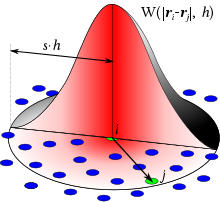
\includegraphics{SPHInterpolationColorsVerbose.png}
\caption{SPH particles and their kernel}
\end{figure}

\href{https://en.wikipedia.org/wiki/Smoothed-particle_hydrodynamics}{Wikipedia}
\textbar{}\href{https://abaqus-docs.mit.edu/2017/English/SIMACAEANLRefMap/simaanl-c-sphanalysis.htm}{MIT}
\textbar{}\href{https://zh.wikipedia.org/wiki/\%E5\%85\%89\%E6\%BB\%91\%E7\%B2\%92\%E5\%AD\%90\%E6\%B5\%81\%E4\%BD\%93\%E5\%8A\%A8\%E5\%8A\%9B\%E5\%AD\%A6}{维基百科}

\begin{enumerate}
\def\labelenumi{\arabic{enumi}.}
\tightlist
\item
  Originally proposed for astrophysical problems
\item
  No mesjes. Very suitable for free-surface flows!
\item
  Easy to understand intuitively: just image each partivle is a small
  parcel of water (although strictly not the case!)
\end{enumerate}

\hypertarget{implenting-sph-using-th-equation-of-states-eos}{%
\paragraph{Implenting SPH using th Equation of States
(EOS)}\label{implenting-sph-using-th-equation-of-states-eos}}

Also known as Weakly Compressible SPH (WCSPH). Momentum equation:
(\(\rho\): density; \(B\): bulk modulus(体积模量); \(\gamma\): constant,
usually \(\sim\) 7)

\begin{equation*}
\begin{array}{rlrl}
\displaystyle\frac{D{\rm v}}{Dt}&=-\displaystyle\frac{1}{\rho}\nabla p+g,
 &p&=B\left(\left(\displaystyle\frac{\rho}{\rho_{0}}\right)^{\gamma}-1\right) \\
A({\rm x})&=\displaystyle\sum_{i}A_{i}\displaystyle\frac{m_{i}}{\rho_{i}}W(||{\rm x - x}_{j}||_{2}, h),
 &\rho_{i}&=\displaystyle\sum_{j}m_{j}W(||{\rm x}_ {i} - {\rm x} _{j}||_{2}, h),
\end{array}
\end{equation*}

Note: the WCSPH paper should have used material derivatives.

\hypertarget{gradients-in-sph}{%
\paragraph{Gradients in SPH}\label{gradients-in-sph}}

\begin{equation*}
\begin{array}{rl}
A({\rm x})&=\displaystyle\sum_{i}A_{i}\displaystyle\frac{m_{i}}{\rho_{i}}W(||{\rm x - x}_{j}||_{2}, h) \\
\nabla A_{i}&=\rho_{i}\displaystyle\sum_{j}m_{j}
               \left(\displaystyle\frac{A_{i}}{\rho_{i}^{2}}+\displaystyle\frac{A_{j}}{\rho_{j}^{2}}\right)
               \nabla_{{\rm x}_{i}} W(||{\rm x}_ {i} - {\rm x} _{j}||_{2}, h)
\end{array}
\end{equation*}

\begin{verbatim}
- Not really accurate...
- but at least symmetric and momentum conserving!
\end{verbatim}

\hypertarget{sph-simulation-cycle}{%
\paragraph{SPH Simulation Cycle}\label{sph-simulation-cycle}}

\begin{enumerate}
\def\labelenumi{\arabic{enumi}.}
\tightlist
\item
  For each particle \(i\), compute
  \(\rho_{i}=\sum_{j}m_{j}W(||{\rm x}_ {i} - {\rm x} _{j}||_{2}, h)\)
\item
  For each particle \(i\), compute \(\nabla p_{i}\) using the gradient
  operator
\item
  Sympletic Euler step (again\ldots):
\end{enumerate}

\begin{equation*}
\begin{array}{rl}
    {\rm v}_ {t+1} &={\rm v}_ {t}+\Delta t\displaystyle\frac{D{\rm v}}{Dt} \\
    {\rm x}_ {t+1} &={\rm x}_ {t}+\Delta t{\rm v}_{t+1}
\end{array}
\end{equation*}

\hypertarget{courant-friedrichs-levy-cfl-condition}{%
\paragraph{Courant-Friedrichs-Levy (CFL)
condition}\label{courant-friedrichs-levy-cfl-condition}}

One upper bound of time step size:

\begin{equation*}
C=\frac{u\Delta t}{\Delta x}\le C_{max}\sim 1
\end{equation*}
\begin{itemize}
  \item \(C\): CFL number (Courant number, or simple the CFL)
  \item \(\Delta t\): time step
  \item \(\Delta x\): length interval (e.g.~particle radius and grid size)
  \item \(u\): maximum (velocity)
\end{itemize}

Application: estimating allowed time step in (explicit) time
integrations. Typical \(C_{max}\) in graphics:
\begin{itemize}
  \item SPH \textasciitilde{} 0.4
  \item MPM: 0.3\textasciitilde 1 
  \item FLIP fluid (smoke): 1\textasciitilde5+
\end{itemize}

\hypertarget{accerating-sph-neighborhood-search}{%
\paragraph{Accerating SPH: Neighborhood
search}\label{accerating-sph-neighborhood-search}}

So far, per substep complexity of SPH is \(O(n^{2})\). This is too
costly to be pratical. In practica, people build spatial data structure
such as voxal grids to accelerate neighborhood search. This reduces time
complexity to \(O(n)\).


    % Add a bibliography block to the postdoc
    
    
    
\end{document}
